% Hoy vamos a crear una presentación con beamer
\documentclass{beamer}

% Vamos a modificar el tema de la presentación
\usetheme{Singapore}
\usecolortheme{rose}
\setbeamertemplate{blocks}[rounded][shadow=true]
\setbeamercovered{invisible}

\usepackage[utf8]{inputenc}
\usepackage[spanish]{babel}
\uselanguage{Spanish}
\languagepath{Spanish}

\usepackage[T1]{fontenc}
\usepackage{FiraSans}

\usepackage{amsthm}
\usepackage{amsmath}
\usepackage{amssymb}
\usepackage{amsfonts}
\usepackage{bbm}
\usepackage{bm}

\usepackage{multicol}
\usepackage{tikz}

\usepackage{wasysym}
\usepackage{url}

% También vamos a aprender a hacer una bibliografía (tipo APA :( )
\usepackage{csquotes}
\usepackage[backend=biber,style=apa]{biblatex}
\DeclareLanguageMapping{spanish}{spanish-apa}
\addbibresource{res.bib}
\urlstyle{same} % Para que los enlaces url no cambien de fuente

\title{Presentaciones en \LaTeX}
\subtitle{Beamer y otras cosas}
\author{inm}
\institute{Taller de \LaTeX}
\logo{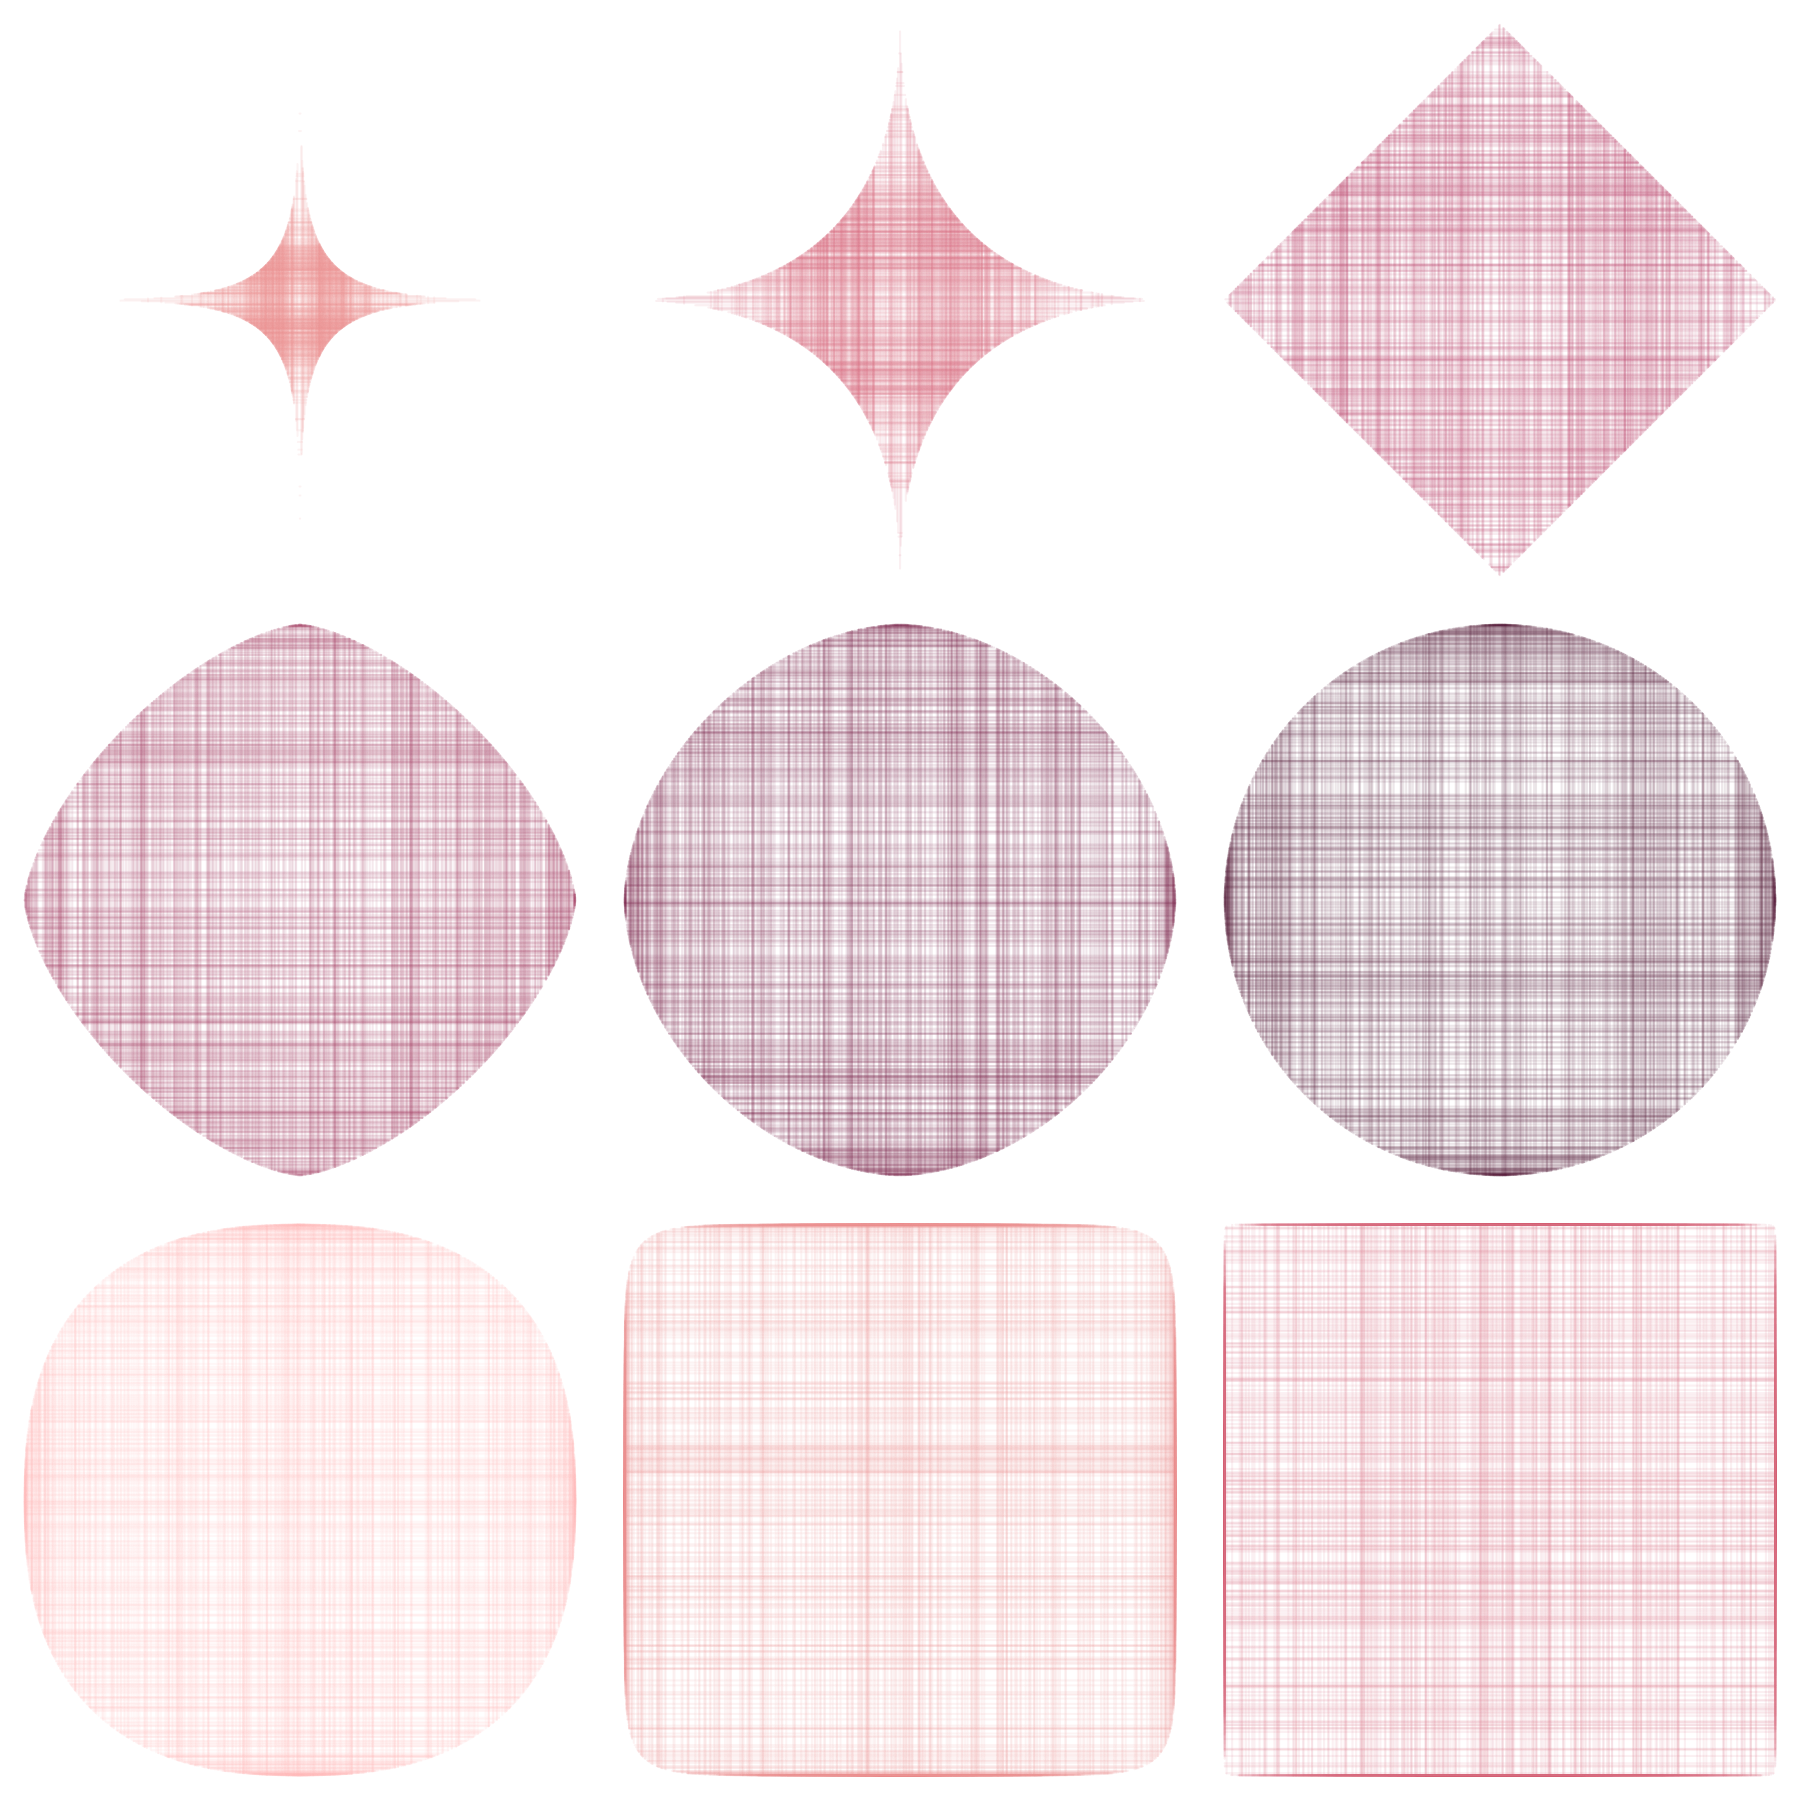
\includegraphics[width=0.5in]{images/98.png}}
% Estamos usando \includegraphics sin haber cargado graphicx

\begin{document}

\begin{frame}
    \maketitle
\end{frame}

\section{El diablo está en los detalles}

\begin{frame}
    \frametitle{Tengo una duda de \LaTeX, ¿qué hago?}

    \begin{enumerate}[<+->]
        \item Llorar.
        \item Identificar su duda.
        \item Escribir nuestra duda lo más específico posible.
        \item Preguntarle a alguien que sepa de \LaTeX. Si sabe, ya acabamos.
        \item ¿Y si no sabe? Llorar de nuevo.
        \item Ir a \url{www.google.com} y buscar las palabras más importantes de nuestra duda.
        \item ¿Está la respuesta en \url{https://tex.stackexchange.com/}? Si sí, ya quedó.
        \item ¿Nada de lo anterior funciona? Plañir porque hay que leer documentación y probablemente código de \LaTeX.
    \end{enumerate}

\end{frame}

\begin{frame}
    \frametitle{¿Cómo se preguntan las dudas de \LaTeX?}

    Cuando comenzamos a usar \LaTeX\ no sabemos preguntar bien las cosas. Algunas recomendaciones:
    \begin{itemize}
        \item Ver si el error es local (es nuestra computadora) o si también sucede en una página como Overleaf.
        \item No enviar fotos de la pantalla, no sirve.
        \item Evitar dudas vagas como ``Me marcó un error''.
        \item Crear un pequeño documento, llamado \textsc{mwe} por \emph{Minimal Working Example}, en el cual se presente un error o en el que pongan lo que han intentado.
        \item Ir a \url{https://tex.stackexchange.com/} y lean las dudas de otros y vean las recomendaciones que dan las personas que responden.
    \end{itemize}

\end{frame}

\begin{frame}
    \frametitle{¿Y si queremos poner dos figuras en una lámina?}

    Vamos a poner dos figuras aquí usando \texttt{minipage}.
    \begin{minipage}[b]{0.45\textwidth}
        \begin{figure}[ht]
            \centering
            \begin{tikzpicture}[scale=1]
                \draw[thick, ->] (0,0) -- (0, 2.2) coordinate[label={right:$z$}];
                \draw[thick, ->] (0,0) -- (2.166577, 0.382026) coordinate[label={right:$y$}];
                \draw[thick, ->] (0,0) -- (1.905256, -1.1) coordinate[label={below:$x$}];
                \draw[thick, dotted] (0, 2) -- (1.9696155, 2.3472964) -- (1.9696155, 0.3472964) -- (3.7016663, -0.6527036) -- (3.701666, 1.347296) -- (1.9696155, 2.3472964);
                \filldraw[thick, draw = black, fill = red, fill opacity = 0.2] (0, 0) -- (1.732051, -1.000000) -- (3.701666, 1.347296) --cycle;
                \filldraw[thick, draw = black, fill = red, fill opacity = 0.2] (0,0) -- (1.9696155, 0.3472964) -- (3.701666, 1.347296) -- cycle;
                \draw[thick, dotted] (0,2) -- (1.732051, 1.000000) -- (1.732051, -1.000000) -- (3.7016663, -0.6527036) -- (3.701666, 1.347296) -- (1.732051, 1.000000);
              \end{tikzpicture}
            \caption{Cota superior de Frechét--Hoeffding}
            \label{fig:frehoeffsup}
        \end{figure}
    \end{minipage}
    ~
    \begin{minipage}[b]{0.45\textwidth}
        \begin{figure}[ht]
            \centering
              \begin{tikzpicture}[scale=1]
                \draw[thick, ->] (0,0) -- (0, 2.2) coordinate[label={right:$z$}];
                \draw[thick, ->] (0,0) -- (2.166577, 0.382026) coordinate[label={right:$y$}];
                \draw[thick, ->] (0,0) -- (1.905256, -1.1) coordinate[label={below:$x$}];
                \draw[thick, dotted] (0, 2) -- (1.9696155, 2.3472964) -- (1.9696155, 0.3472964) -- (3.7016663, -0.6527036) -- (3.701666, 1.347296) -- (1.9696155, 2.3472964);
                \filldraw[thick, draw = black, fill = blue, fill opacity = 0.2] (0, 0) -- (1.732051, -1.000000) -- (1.9696155, 0.3472964) --cycle;
                \filldraw[thick, draw = black, fill = blue, fill opacity = 0.2] (1.732051, -1.000000) -- (1.9696155, 0.3472964) -- (3.701666, 1.347296) -- cycle;
                \draw[thick, dotted] (0,2) -- (1.732051, 1.000000) -- (1.732051, -1.000000) -- (3.7016663, -0.6527036) -- (3.701666, 1.347296) -- (1.732051, 1.000000);
              \end{tikzpicture}
            \caption{Cota inferior de Frechét--Hoeffding.}
            \label{fig:frehoeffinf}
          \end{figure}
    \end{minipage}

\end{frame}

\begin{frame}
    \frametitle{Podemos poner una figura y texto en una misma lámina}

    \begin{minipage}[b]{0.3\textwidth}
        \begin{figure}[ht]
            \centering
            
\includegraphics[width = \textwidth]{images/81.png}
            \caption{Una figura hecha en \textsc{r}.}
            \label{fig:mi figura}
        \end{figure}
    \end{minipage}
    ~
    \begin{minipage}[b]{0.65\textwidth}
        Escribamos una breve lista sin sentido.
        \begin{enumerate}
            \item Hola
            \item mundo
            \item es
            \item la 
            \item cosa
            \item más
            \item inútil.
        \end{enumerate}
    \end{minipage}

\end{frame}

\begin{frame}[allowframebreaks]
    \frametitle{¿Y si me piden citar en APA?}

    \begin{enumerate}
        \item Llorar.
        \item Huir, no hay nada peor que hacerle caso a los psicológos. 
        \item Resignarnos porque no nos queda de otra.
        \item Crear un archivo .bib en el que vamos a meter toooooodas las referencia que usemos. Un pequeño ejemplo de cómo son los elementos del archivo .bib es el siguiente.
        \begin{center}
            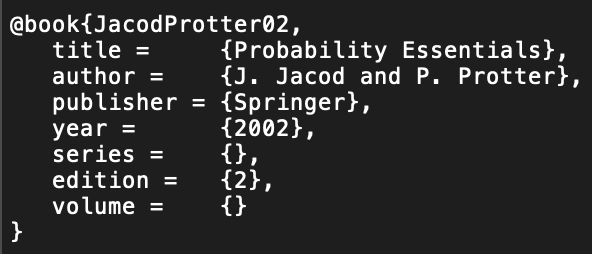
\includegraphics[height=1in]{images/ejemplo.png}
        \end{center}
        \item Incluir la línea \texttt{\textbackslash{}usepackage[backend=biber]\{biblatex\}} esperando a que no nos obliguen a usar APA.
        \item Si APA es importantísimo, lloramos y hay que cargar \texttt{biblatex} con la opción \texttt{style = apa}.
        \item Agregar al preámbulo la línea \texttt{\textbackslash{}DeclareLanguageMapping\{spanish\}\{spanish-apa\}}.
        \item Cargar el archivo .bib con la línea \texttt{\textbackslash{}addbibresource\{res.bib\}}
        \item Citar algún documento, ejemplo: \texttt{\textbackslash{}cite\{Etemadi81\}} imprime \cite{Etemadi81}. Otro ejemplo: \cite{Norris97}.
        \item Imprimir la bibliografía o referencias con el comando \texttt{\textbackslash{}printbibliography}.
        \item Entregar un trabajo impecable.
    \end{enumerate}

\end{frame}

\section{Algunas otras cosas}

\begin{frame}
    \frametitle{Caaaaaaaajas}

    \begin{block}{Este es un bloque}<1->
        Y aquí hay información que debemos remarcar.
    \end{block}

    \begin{alertblock}<3->{Alerta alerta}
        Ya no sé qué más escribir.
    \end{alertblock}

    \begin{exampleblock}<2->{Esto es un ejemplo}
        Esto no es un ejemplo.
    \end{exampleblock}

\end{frame}

\begin{frame}
    \frametitle{Más cajitasss}

    \begin{definition}
        Soy una definición. :P
    \end{definition} \pause

    \begin{theorem}[del mago Chen Kai]
        Soy un teorema.
    \end{theorem} \pause

    \begin{corollary}
        Y yo soy un corolario.
    \end{corollary} \pause

    \begin{proof}
        Aquí se prueban cosas.
    \end{proof}

\end{frame}

\begin{frame}[t]
    \frametitle{Pruebas}

    \begin{exampleblock}{hola}
        hola
    \end{exampleblock}

\end{frame}

\begin{frame}
    \frametitle{Referencias}

    \printbibliography

\end{frame}

\end{document}